\documentclass{article}
\usepackage{template}

\usepackage{chngcntr} % Reset counter within sections

\counterwithin*{equation}{section}
\counterwithin*{equation}{subsection}

\pagestyle{fancy}
\setlength\headheight{24pt}

\lhead{\docTitle}
\rhead{\leftmark}
\cfoot{\thepage}

\newcommand{\docTitle}{Trigonometry }

\usepackage[
    type={CC},
    modifier={by-nc-sa},
    version={4.0},
    imagewidth={5em},
]{doclicense}

\date{}

\begin{document}
\begin{titlepage}
    \vspace*{\fill}
    \begin{center}
        \LARGE
        \textbf{\docTitle}
    \end{center}
    \vspace*{\fill}
    \doclicenseThis
    \thispagestyle{empty}
\end{titlepage}
\newpage

\tableofcontents
\newpage

\renewcommand*{\arraystretch}{1.25}
\section{Definitions}
\subsection{Trigonometric Functions}
\begin{figure}[H]
    \centering
    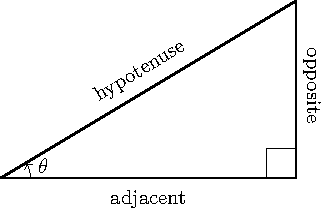
\includegraphics[height = 4cm, keepaspectratio = true]{right triangle}
\end{figure}
\begin{align*}
    \sin{\left( \theta \right)} &= \frac{\text{opposite}}{\text{hypotenuse}} & \csc{\left( \theta \right)} &= \frac{\text{hypotenuse}}{\text{opposite}} \\
    \cos{\left( \theta \right)} &= \frac{\text{adjacent}}{\text{hypotenuse}} & \sec{\left( \theta \right)} &= \frac{\text{hypotenuse}}{\text{adjacent}} \\
    \tan{\left( \theta \right)} &= \frac{\text{opposite}}{\text{adjacent}}   & \cot{\left( \theta \right)} &= \frac{\text{adjacent}}{\text{opposite}} 
\end{align*}
\subsection{Inverse Trigonometric Functions}
\begin{align*}
    y=\arccos{\left( x \right)} &\iff x=\cos{\left( y \right)} & y=\arccsc{\left( x \right)} &\iff x=\csc{\left( y \right)} \\
    y=\arcsin{\left( x \right)} &\iff x=\sin{\left( y \right)} & y=\arcsec{\left( x \right)} &\iff x=\sec{\left( y \right)} \\
    y=\arctan{\left( x \right)} &\iff x=\tan{\left( y \right)} & y=\arccot{\left( x \right)} &\iff x=\cot{\left( y \right)}
\end{align*}
\subsection{Domain and Range}
Let $n\in\mathbb{Z}$ be a constant.
\begin{table}[H]
	\centering
	\begin{tabular}{>{$}c<{$}|>{$}c<{$}>{$}c<{$}}
		\toprule
		\text{Function} & \text{Domain} & \text{Range} \\
		\midrule
		\sin{\left( x \right)} & \mathbb{R}                                                          & \left[-1,\:1\right] \\
		\cos{\left( x \right)} & \mathbb{R}                                                          & \left[-1,\:1\right] \\
		\tan{\left( x \right)} & \mathbb{R}\backslash\Bigl\{ \left( n+\frac{1}{2} \right)\pi \Bigr\} & \mathbb{R} \\
		\cot{\left( x \right)} & \mathbb{R}\backslash\Bigl\{ n\pi \Bigr\}                            & \mathbb{R} \\
		\sec{\left( x \right)} & \mathbb{R}\backslash\Bigl\{ \left( n+\frac{1}{2} \right)\pi \Bigr\} & \left(-\infty,\:-1\right]\cup\left[1,\:\infty\right) \\
		\csc{\left( x \right)} & \mathbb{R}\backslash\Bigl\{ n\pi \Bigr\}                            & \left(-\infty,\:-1\right]\cup\left[1,\:\infty\right) \\
		\bottomrule
	\end{tabular}
\end{table}
\begin{table}[H]
	\centering
	\begin{tabular}{>{$}c<{$}|>{$}c<{$}>{$}c<{$}}
		\toprule
		\text{Function} & \text{Domain} & \text{Range} \\
		\midrule
		\arcsin{\left( x \right)} & \left[-1,\:1\right]                                  & \left[-\frac{\pi}{2},\:\frac{\pi}{2}\right] \\
		\arccos{\left( x \right)} & \left[-1,\:1\right]                                  & \left[0,\:\pi\right] \\
		\arctan{\left( x \right)} & \mathbb{R}                                           & \left[-\frac{\pi}{2},\:\frac{\pi}{2}\right] \\
		\arccot{\left( x \right)} & \mathbb{R}                                           & \left[0,\:\pi\right] \\
		\arcsec{\left( x \right)} & \left(-\infty,\:-1\right]\cup\left[1,\:\infty\right) & \left[0,\:\pi\right]\backslash\left\{ \frac{\pi}{2} \right\} \\
		\arccsc{\left( x \right)} & \left(-\infty,\:-1\right]\cup\left[1,\:\infty\right) & \left[-\frac{\pi}{2},\:\frac{\pi}{2}\right]\backslash\left\{ 0 \right\} \\
		\bottomrule
	\end{tabular}
\end{table}
\section{Identities}
\subsection{Pythagorean Identities}
\begin{equation*}
	\sin^2{\left( x \right)} + \cos^2{\left( x \right)} = 1
\end{equation*}
Dividing by either the sine or cosine function gives:
\begin{align*}
	\tan^2{\left( x \right)} + 1 &= \sec^2{\left( x \right)} \\
	1 + \cot^2{\left( x \right)} &= \csc^2{\left( x \right)}
\end{align*}
\subsection{Symmetry Identities}
\begin{align*}
		\sin{\left( -x \right)} &= -\sin{\left( x \right)} & \csc{\left( -x \right)} &= -\csc{\left( x \right)} \\
		\cos{\left( -x \right)} &=  \cos{\left( x \right)} & \sec{\left( -x \right)} &=  \sec{\left( x \right)} \\
		\tan{\left( -x \right)} &= -\tan{\left( x \right)} & \cot{\left( -x \right)} &= -\cot{\left( x \right)}
\end{align*}
\subsection{Periodicity Identities}
\begin{align*}
    \sin{\left( x+2\pi n \right)} &= \sin{\left( x \right)} & \csc{\left( x+2\pi n \right)} &= \csc{\left( x \right)} \\
    \cos{\left( x+2\pi n \right)} &= \cos{\left( x \right)} & \sec{\left( x+2\pi n \right)} &= \sec{\left( x \right)} \\
    \tan{\left( x+\pi n \right)}  &= \tan{\left( x \right)} & \cot{\left( x+\pi n \right)}  &= \cot{\left( x \right)}
\end{align*}
\subsection{Angle Sum Identities}
\begin{align*}
	\sin{\left( x\pm y \right)} &= \sin{\left( x \right)} \cos{\left( y \right)} \pm \cos{\left( x \right)} \sin{\left( y \right)}           & \csc{\left( x\pm y \right)} &= \frac{1}{\sin{\left( x \right)} \cos{\left( y \right)} \pm \cos{\left( x \right)} \sin{\left( y \right)}} \\
	\cos{\left( x\pm y \right)} &= \cos{\left( x \right)} \cos{\left( y \right)} \mp \sin{\left( x \right)} \sin{\left( y \right)}           & \sec{\left( x\pm y \right)} &= \frac{1}{\cos{\left( x \right)} \cos{\left( y \right)} \mp \sin{\left( x \right)} \sin{\left( y \right)}} \\
	\tan{\left( x\pm y \right)} &= \frac{\tan{\left( x \right)}\pm\tan{\left( y \right)}}{1\mp \tan{\left( x \right)}\tan{\left( y \right)}} & \cot{\left( x\pm y \right)} &= \frac{\cot{\left( x \right)}\cot{\left( y \right)}\mp 1}{\cot{\left( x \right)}\pm\cot{\left( y \right)}}   
\end{align*}
\subsection{Double-Angle Identities}
\begin{align*}
	\sin{\left( 2x \right)} &= 2\sin{\left( x \right)}\cos{\left( x \right)}              & \csc{\left( 2x \right)} &= \frac{1}{2}\sec{\left( x \right)}\csc{\left( x \right)} \\
	\cos{\left( 2x \right)} &= \cos^2{\left( x \right)} \sin^2{\left( x \right)}          & \sec{\left( 2x \right)} &= \frac{\sec^2{\left( x \right)}\csc^2{\left( x \right)}}{\csc^2{\left( x \right)}-\sec^2{\left( x \right)}} \\
	\tan{\left( 2x \right)} &= \frac{2\tan{\left( x \right)}}{1-\tan^2{\left( x \right)}} & \cot{\left( 2x \right)} &= \frac{\cot^2{\left( x \right)}-1}{2\cot{\left( x \right)}} 
\end{align*}
\subsection{Power Reducing Identities}
\begin{align*}
	\sin^2{\left( x \right)} &= \frac{1}{2}\bigl( 1-\cos{\left( 2x \right)} \bigr)          & \csc^2{\left( x \right)} &= \frac{2}{1-\cos{\left( 2x \right)}} \\
	\cos^2{\left( x \right)} &= \frac{1}{2}\bigl( 1+\cos{\left( 2x \right)} \bigr)          & \sec^2{\left( x \right)} &= \frac{2}{1+\cos{\left( 2x \right)}} \\
	\tan^2{\left( x \right)} &= \frac{1-\cos{\left( 2x \right)}}{1+\cos{\left( 2x \right)}} & \cot^2{\left( x \right)} &= \frac{1+\cos{\left( 2x \right)}}{1-\cos{\left( 2x \right)}}
\end{align*}
\subsection{Half Angle Identities}
\begin{align*}
	\sin{\left( \frac{x}{2} \right)} &= \left( -1 \right)^{\floor{\frac{x}{2\pi}}}\sqrt{\frac{1}{2}\bigl(1-\cos{\left( x \right)}\bigr)}     & \csc{\left( \frac{x}{2} \right)} &= \pm \sqrt{\frac{2\sec{\left( x \right)}}{\sec{\left( x \right)}-1}} \\
	\cos{\left( \frac{x}{2} \right)} &= \left( -1 \right)^{\floor{\frac{x+\pi}{2\pi}}}\sqrt{\frac{1}{2}\bigl(1+\cos{\left( x \right)}\bigr)} & \sec{\left( \frac{x}{2} \right)} &= \pm \sqrt{\frac{2\sec{\left( x \right)}}{\sec{\left( x \right)}+1}} \\
	\tan{\left( \frac{x}{2} \right)} &= \frac{1-\cos{\left( x \right)}}{\sin{\left( x \right)}}                                              & \cot{\left( \frac{x}{2} \right)} &= \frac{\sin{\left( x \right)}}{1-\cos{\left( x \right)}} 
\end{align*}
\subsection{Werner Identities}
\begin{align*}
	 2\sin{\left( x \right)}\sin{\left( y \right)} &= \cos{\left( x-y \right)}-\cos{\left( x+y \right)} \\
	 2\cos{\left( x \right)}\cos{\left( y \right)} &= \cos{\left( x-y \right)}+\cos{\left( x+y \right)} \\
	 2\sin{\left( x \right)}\cos{\left( y \right)} &= \sin{\left( x-y \right)}+\sin{\left( x+y \right)} \\
    -2\cos{\left( x \right)}\sin{\left( y \right)} &= \sin{\left( x-y \right)}-\sin{\left( x+y \right)}
\end{align*}
\subsection{Prosthaphaeresis Identities}
\begin{align*}
	\sin{\left( x \right)}+\sin{\left( y \right)} &= 2\sin{\left(\frac{1}{2} \left( x+y \right) \right)}\cos{\left( \frac{1}{2} \left( x-y \right) \right)} \\
	\sin{\left( x \right)}-\sin{\left( y \right)} &= 2\cos{\left(\frac{1}{2} \left( x+y \right) \right)}\sin{\left( \frac{1}{2} \left( x-y \right) \right)} \\
	\cos{\left( x \right)}+\cos{\left( y \right)} &= 2\cos{\left(\frac{1}{2} \left( x+y \right) \right)}\cos{\left( \frac{1}{2} \left( x-y \right) \right)} \\
	\cos{\left( x \right)}-\cos{\left( y \right)} &= -2\sin{\left(\frac{1}{2} \left( x+y \right) \right)}\sin{\left( \frac{1}{2} \left( x-y \right) \right)} \\
\end{align*}
\subsection{Inverse Reciprocal Identities}
\begin{align*}
    \arcsin{\left( \frac{1}{x} \right)} &= \arccsc{\left( x \right)} & \arccsc{\left( \frac{1}{x} \right)} &= \arcsin{\left( x \right)} \\
    \arccos{\left( \frac{1}{x} \right)} &= \arcsec{\left( x \right)} & \arcsec{\left( \frac{1}{x} \right)} &= \arccos{\left( x \right)} \\
    \arctan{\left( \frac{1}{x} \right)} &= \arccot{\left( x \right)} & \arccot{\left( \frac{1}{x} \right)} &= \arctan{\left( x \right)} \\
\end{align*}
\section{Triangle Identities}
\begin{figure}[H]
	\centering
	\includegraphics*{triangle.pdf}
\end{figure}
\subsection{Area of a Triangle}
\begin{equation}
	A=\frac{1}{2}a b \sin{\left( \gamma \right)}
\end{equation}
\subsection{Sine Rule}
\begin{equation}
	\frac{\sin{\left( \alpha \right)}}{a} = \frac{\sin{\left( \beta \right)}}{b} = \frac{\sin{\left( \gamma \right)}}{c}
\end{equation}
\subsection{Cosine Rule}
\begin{equation}
	a^2=b^2+c^2-2b c\cos{\left( \alpha \right)}
\end{equation}
\subsection{Tangent Rule}
\begin{equation}
	\frac{\tan{\left( \frac{1}{2}\left( \alpha-\beta \right) \right)}}{\tan{\left( \frac{1}{2}\left( \alpha+\beta \right) \right)}} = \frac{a-b}{a+b}
\end{equation}
\subsection{Mollweide's Identity}
\begin{equation}
	\frac{b-c}{a}=\frac{\sin{\left( \frac{1}{2}\left( \beta-\gamma \right) \right)}}{\cos{\left( \frac{\alpha}{2} \right)}}
\end{equation}
\subsection{Newton's Identity}
\begin{equation}
	\frac{b+c}{a}=\frac{\cos{\left( \frac{1}{2}\left( \beta-\gamma \right) \right)}}{\sin{\left( \frac{\alpha}{2} \right)}}
\end{equation}
\end{document}